  \begin{tikzpicture}
  \node[anchor=south west,inner sep=0] (image) at (0,0,0) 
  {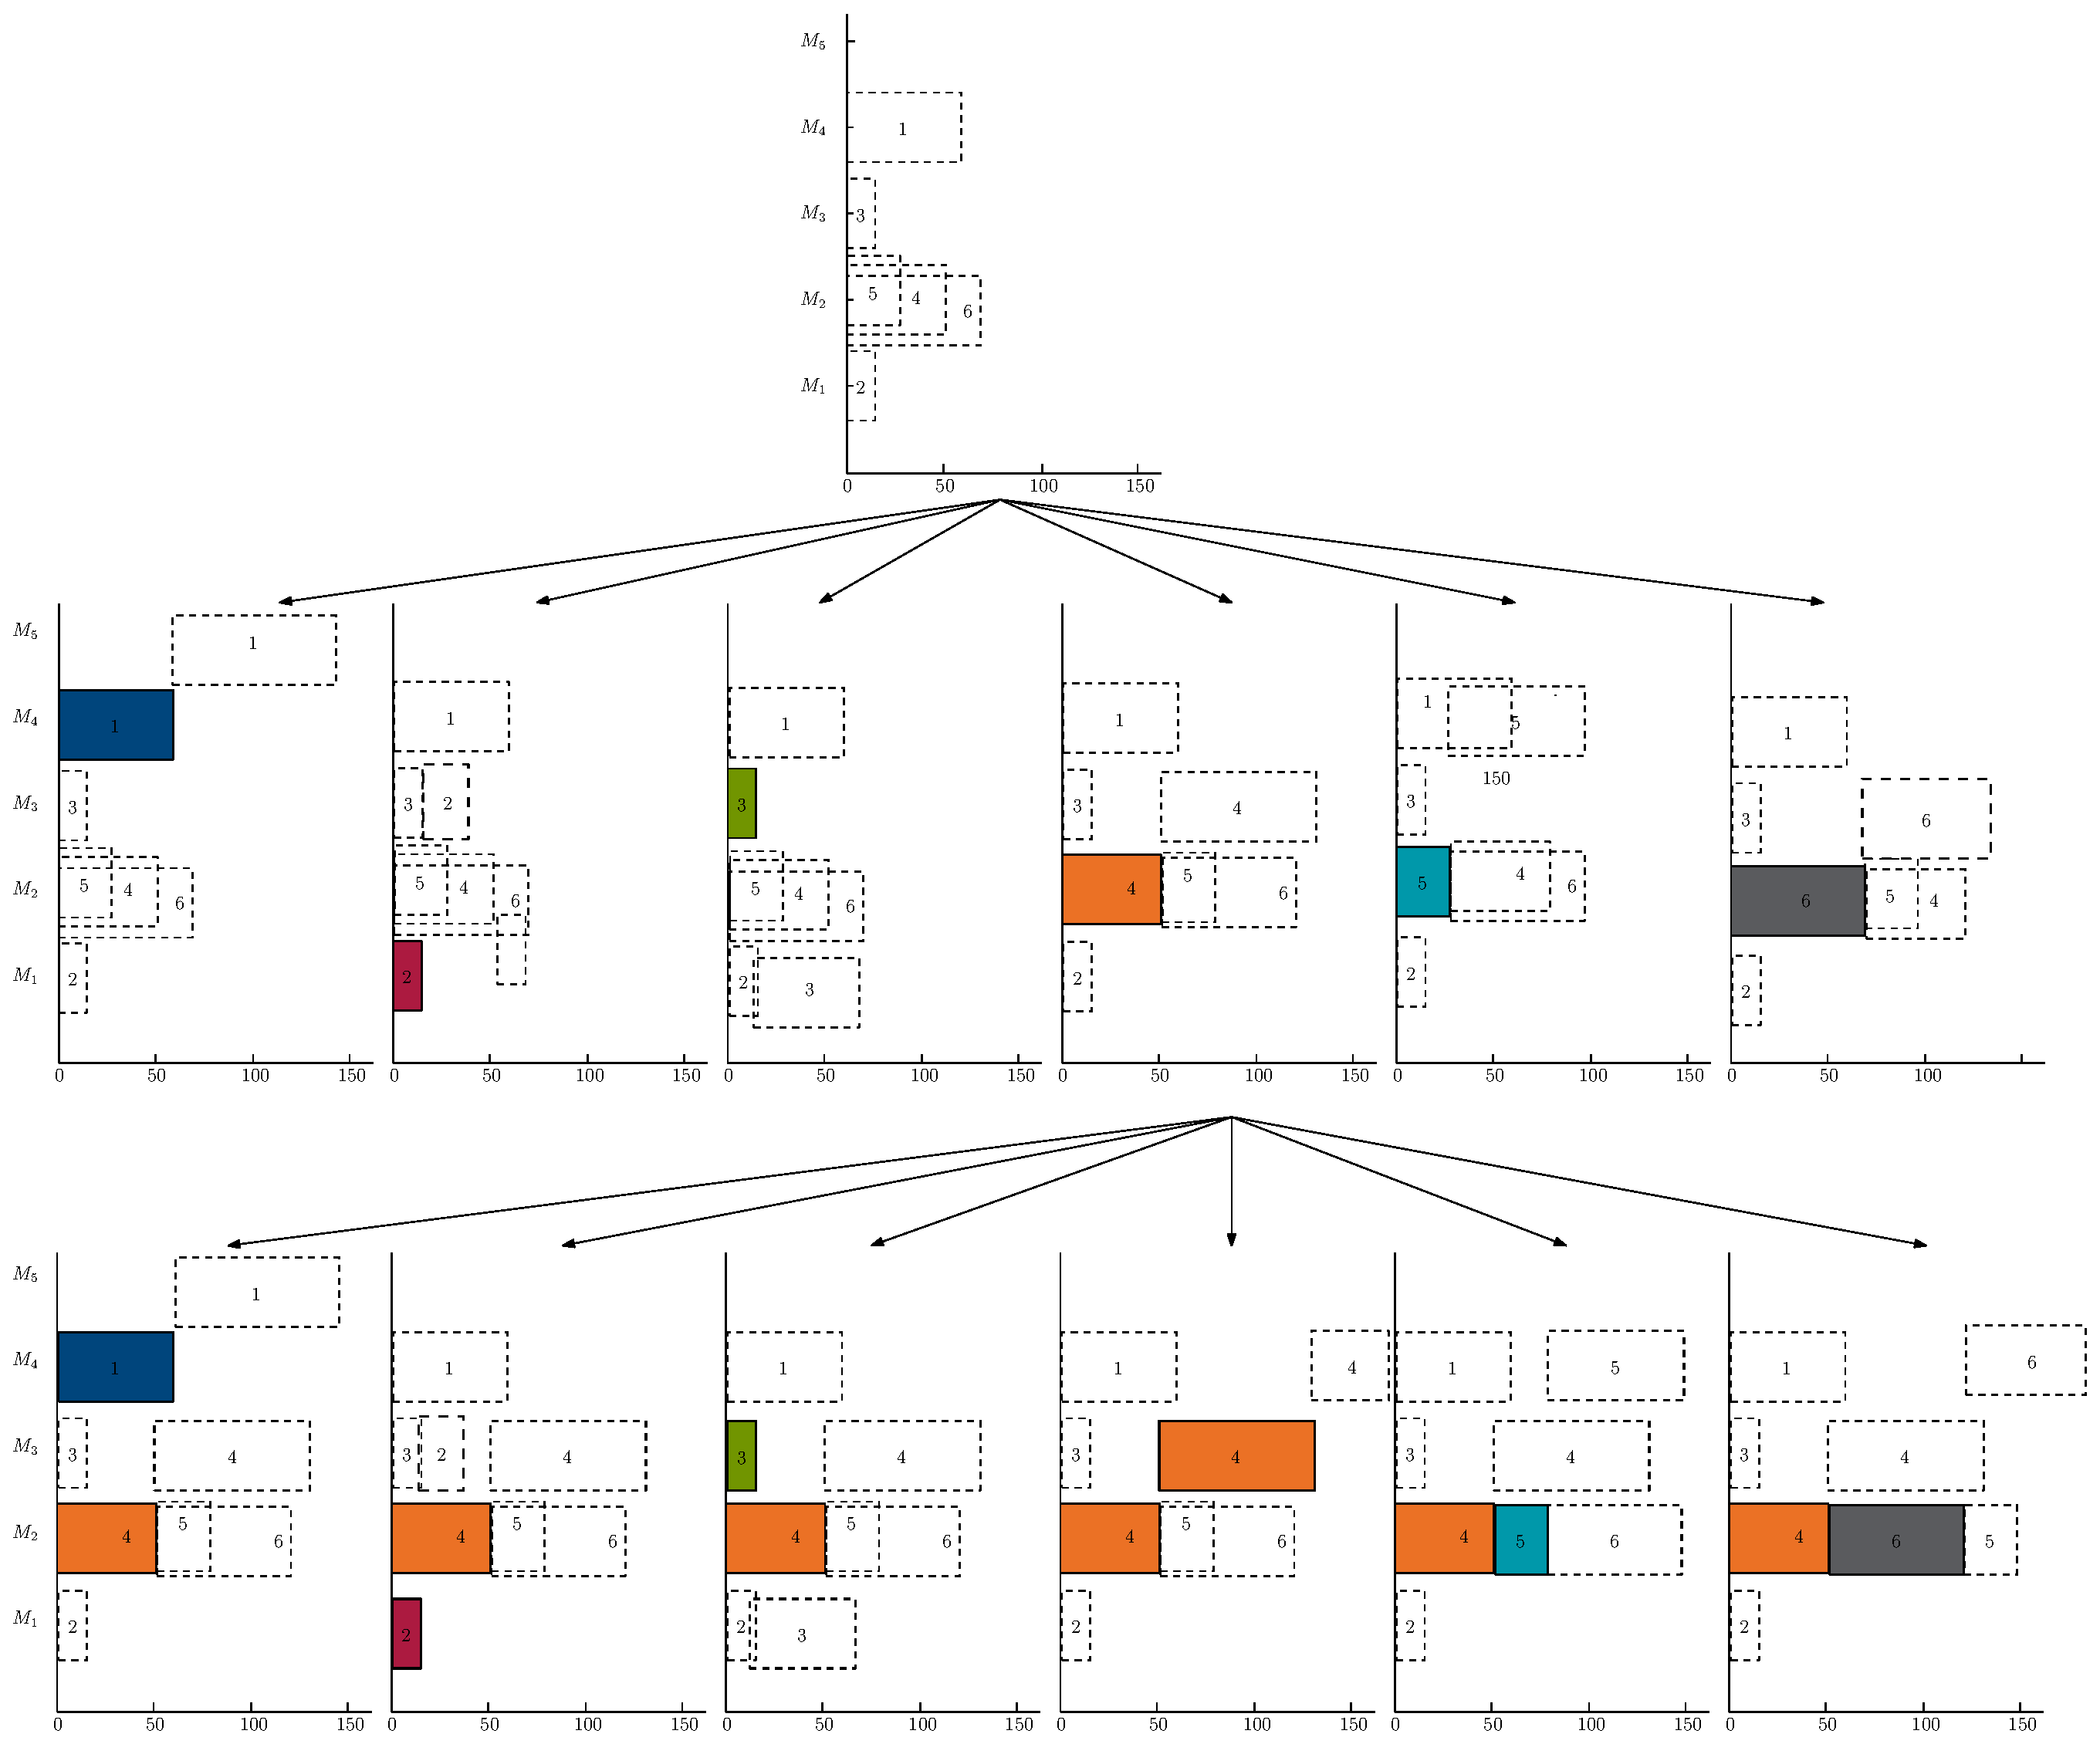
\includegraphics[width=\textwidth]{gametree}};
  \begin{scope}[x={(image.south east)},y={(image.north west)}]
  %% next four lines will help you to locate the point needed by forming a 
  %%grid. comment these four lines in the final picture.↓
  %\draw[help lines,xstep=.1,ystep=.1] (0,0) grid (1,1);
  %\draw[help lines,xstep=.05,ystep=.05] (0,0) grid (1,1);
  %\foreach \x in {0,1,...,9} { \node [anchor=north] at (\x/10,0) {0.\x}; }
  %\foreach \y in {0,1,...,9} { \node [anchor=east] at (0,\y/10) {0.\y};}
  %% upto here↑
  \node (J0) at (0.5,0.71) {};
  \node (J1) at (0.19,0.65) {};
  \node (J2) at (0.42,0.65) {};
  \node (J3) at (0.65,0.65) {};
  \node (J4) at (0.85,0.65) {};
  \draw[-latex] (J0) to[out=-20,in=+20] (J1);
  \draw[-latex] (J0) to[out=-20,in=+20] (J2);
  \draw[-latex] (J0) to[out=-20,in=+20] (J3);
  \draw[-latex] (J0) to[out=-20,in=+20] (J4);
  \node (J4) at (0.82,0.38) {};
  \node (J4J1) at (0.19,0.31) {};
  \node (J4J2) at (0.42,0.31) {};
  \node (J4J3) at (0.65,0.31) {};
  \node (J4J4) at (0.85,0.31) {};
  \draw[-latex] (J4) to[out=-20,in=+20] (J4J1);
  \draw[-latex] (J4) to[out=-20,in=+20] (J4J2);
  \draw[-latex] (J4) to[out=-20,in=+20] (J4J3);
  \draw[-latex] (J4) to[out=-20,in=+20] (J4J4);
  \end{scope}
  \end{tikzpicture}
